\begin{frame}{Evolutionary neural networks}
    \begin{itemize}
        \item Starting with a set of random configurations
        \vspace{0.2cm}
        \item Evaluate the results of the first generation and generate a new generation based on 
        \vspace{0.2cm}
        \item Repeat until a good configuration is reached
        \vspace{0.2cm}
        \item Advantages:
            \begin{itemize}
                \item Decrease user bias for hyperparameter choice
                \item Optimised to run on worker nodes
                \item Quick discarding of bad configurations
                \item User friendly for unexperienced students
            \end{itemize}
    \end{itemize}
\end{frame}

\begin{frame}{Inner product}
    \begin{equation*}
        a^{\mu} = \begin{pmatrix}
            p_T \cosh ( \eta ) \\
            p_T \cos ( \phi ) \\
            p_T \sin ( \phi ) \\
            p_T \sinh ( \eta ) \end{pmatrix}
    \end{equation*}
    %
    \begin{align*}
        \langle A | B \rangle = A_{\mu} B^{\mu}\\
        = p_{T,A} p_{T,B} ( \cosh ( \eta_A ) \cosh ( \eta_B ) - \cos ( \phi_A ) \cos ( \phi_B)\\
        - \sin ( \phi_A ) \sin ( \phi_B ) -\sinh ( \eta_A ) \sinh ( \eta_B ) )\\
        = p_{T,A} p_{T,B} \left( \cosh ( \eta_A - \eta_B ) - \cos ( \phi_A - \phi_B ) \right)
    \end{align*}
\end{frame}

\begin{frame}{Background processes in neural network training}
    \begin{columns}
        \begin{column}{0.5\textwidth}
            \begin{figure}
                \centering
                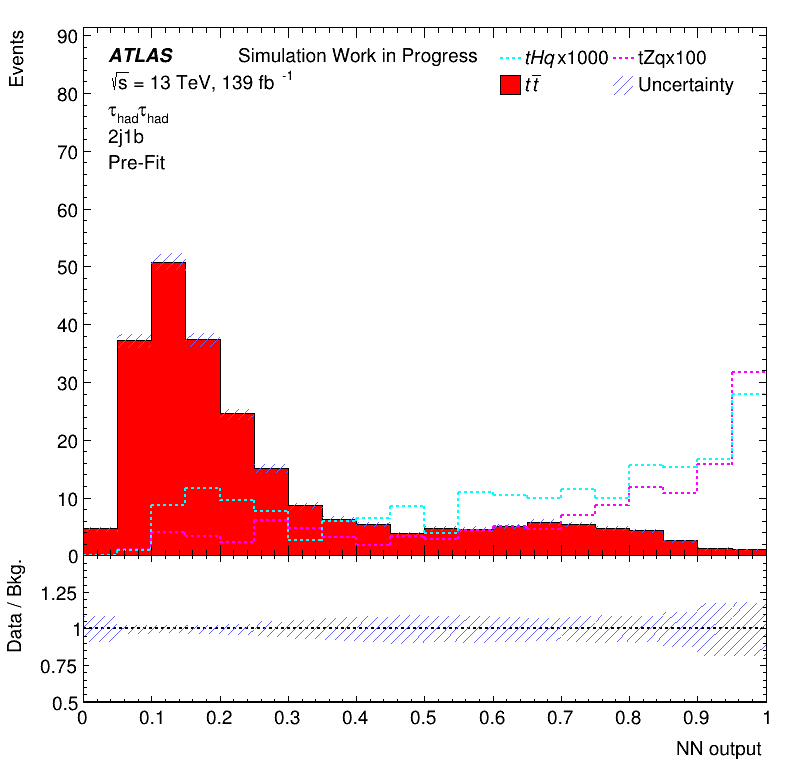
\includegraphics[width=\textwidth]{sgBkgComp}
            \end{figure}
        \end{column}
        \begin{column}{0.5\textwidth}
            \begin{itemize}
                \item tHq against other processes
                \vspace{0.5cm}
                \item ttbar dominates the training
                \vspace{0.5cm}
                \item tZq misclassified as signal
                \vspace{0.5cm}
                \item Possible approaches:
                    \begin{itemize}
                        \item multiple networks
                        \item multiple targets
                        \item reweighting samples
                    \end{itemize} 
            \end{itemize}
        \end{column}
    \end{columns}
\end{frame}

\begin{frame}{General ML selection}
  \begin{columns}
    \begin{column}{0.5\textwidth}
      \centering 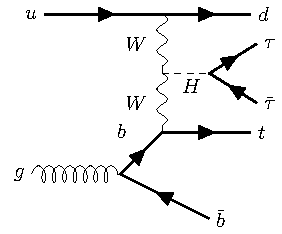
\includegraphics[width=0.45\textwidth]{/cephfs/user/s6chkirf/feynman_diagrams/tHq_tautau}\\
      \includegraphics[width=0.45\textwidth]{/cephfs/user/s6chkirf/feynman_diagrams/tHq_WW}
      \includegraphics[width=0.45\textwidth]{/cephfs/user/s6chkirf/feynman_diagrams/tHq_ZZ}
      \begin{itemize}
        \item n-jets: 2 (b-jets: \textbf{1})
        \item b-jet WP: 70 DL1r
        \item nLeptons \& nTaus: $\bf{1e / \mu~2\tau_{\text{had}}} $
        \item $E_{\text{T,miss}}$: no cut (to \SI{800}{GeV})
      \end{itemize}
    \end{column}
    \begin{column}{0.7\textwidth}
      \vspace*{-0.05\textwidth}
      \begin{itemize}
        \footnotesize
        \item jets:
        \vspace*{-0.02\textwidth}
        \begin{itemize}
          \footnotesize
          \item $p_T>\SI{35}{GeV}$
          \item $|\eta|<4.5$
          \item EMPFlow
        \end{itemize}
        \item electrons:
        \vspace*{-0.02\textwidth}
        \begin{itemize}
          \footnotesize
          \item $p_T>\SI{20}{GeV}$ leading \SI{27}{GeV}
          \item $|\eta|<2.5$ not in 1.37 - 1.52
          \item WP: LooseAndBLayerLH ; \\isolation: no requirement
        \end{itemize}
        \item muons:
        \vspace*{-0.02\textwidth}
        \begin{itemize}
          \footnotesize
          \item $p_T>\SI{20}{GeV}$ leading \SI{27}{GeV}
          \item $0.01<|\eta|<2.5$
          \item WP: Loose ; isolation: no requirement
        \end{itemize}
        \item taus:
        \vspace*{-0.02\textwidth}
        \begin{itemize}
          \footnotesize
          \item $p_T>\SI{20}{GeV}$ leading \SI{27}{GeV}
          \item $|\eta|<2.5$ not in 1.37 - 1.52
          \item WP: RNNLoose
          \item ASG recommended OLR ($\tau_{had}$ remove jets)
        \end{itemize}
      \end{itemize}
    \end{column}
  \end{columns}
\end{frame}

\begin{frame}
    \begin{enumerate}
        \item Understand impact of negative weights on variable shape
        \item Investigate variable shapes for different treatments
        \item Understand impact of negative weights in ML algorithms
        \item Test different approaches for negative weight handling and investigate the model stability.
    \end{enumerate}
\end{frame}